\documentclass[../rapport.tex]{subfiles}

\begin{document}
    \chapter{Le stage}
    \section{Sujet}
        Durant mon stage, j'ai eu l'occasion de travailler sur 3 projets successif.
        Cette alternance de projet m'a permis d'avoir des methodes de travail variées,
        et de ne pas me limiter à une seule technologie.

        J'ai eu ainsi l'occasion de travailler avec par exemple Symfony,
        Laravel, NodeJS, Docker, Typescript, RabbitMQ, MongoDB et MySQL.

        \subsection{Premier projet}
        Le premier projet sur lequel j'ai eu l'occasion de travailler visait à
        développer une application permettant de trouver du travail. Cette
        application destinée au marché asiatique était similaire à jobteaser ou
        linkedin. Je suis arrivé à la fin du développement de ce projet, et j'ai du 
        ajouter des fonctionnalité à l'\gls{api}. Celà à représenté environ un quart de mon
        stage.

        \subsection{Deuxième projet}
        Une fois le premier projet fini, j'ai été assigné à un projet de
        réécriture de micro service. 
        Le projet était commandé par SITA, et il fallait reconcevoir l'implémentation
        de certains micro services sur un de leur projet porté sur les objets
        connectés.
        Ce projet a été l'occasion pour moi de travailler en autonomie, et il a
        constitué également un quart de mon stage.

        \subsection{Troisième projet}
        Le troisième projet consistait à developper une application permettant
        de faciliter la mise en relation de voisin pour tout type de service, comme
        le baby sitting, les course, etc. Pour cette application j'ai dû travailler en
        équipe avec un autre stagiaire, ce projet a donc été pour nous de développer 
        nos compétences collaboratives afin de réaliser cette application.
    \section{Role}
        Dans ces trois projets, j'ai endossé le rôle de développeur côté
        serveur. C'est à dire que je me suis occupé du traitement des données,
        leur stockage, leur validation et le controle de leurs accès etc.
    \section{Déroulement}
        \subsection{Jobigo}\label{subsec:jobigo}
        Au tout début de mon stage, j'ai été assigné à un projet déjà en cours~:~Jobigo.\
        l'objectif de
        ce projet était de permettre de trouver du travail plus facilement
        en mettant en relation chercheur d'emploi, et employeurs.
        Le projet était quasiment terminé au moment où je suis arrivé, il s'agissait simplement d'ajouter
        les derniers détails pour que l'\gls{api} puisse interagir avec l'application mobile
        de façon optimale.
        Pendant Ce projet, je me suis principalement occupé de mettre en place les \glspl{push}.
        Je n'avais pas de connaissances concernants les \glspl{push}, il a donc fallu que 
        j'apprenne en autonomie le principe de fonctionnement, avec notamment l'enregistrement 
        des \glspl{token}. On peut trouver deux types de \glspl{token}: ceux de Apple, et de Google.
        Ceux de apple sont par exemple plus compliqué à utiliser car ils nécessitent la génération 
        de certificats.

            L'api de jobigo a été principalement construite en utilisant php, avec \textit{Api platform}\footnote{https://api-platform.com/} un \gls{framework} permettant de simplifier la conception des \gls{api}.

        Le processus de création d'une \gls{api} implique de pouvoir lister toutes les actions 
        qu'il sera possible de réaliser sur l'application, comme par exemple, la connexion d'un utilisateur, 
        ou la création d'une offre d'emploi dans le cadre de jobigo.

        Il existe des conventions pour concevoir une API, comme la convention \gls{rest} qui a été utilisée
        sur ce projet, mais également sur mynabes\footnote{cf page \pageref{subsec:mynabes}}.

        \subsubsection{Architecture du projet}
        Le projet à été construit autour du framework API platform. Comme la plupart des framework, il applique le pattern \gls{mvc},
        afin d'avoir une architecture evolutive, et surtout maintenable. Dans le cadre de jobigo, cette architecture peut-être résumé comme dans la figure \ref{fig:jobigo}.
        En réalité, toutes les actions que l'on peut faire sur un site web se font au travers d'un controller, et lorsque l'on explore un site web, il y a un jeu de question/réponse entre l'ordinateur et le serveur qui héberge le site. Dans le cadre de Jobigo, il ne s'agit pas d'un ordinateur, mais d'une application qui envoie des requête au serveur.

        Le controleur que l'on peut voir sur la figure \ref{fig:jobigo} est donc le point d'entrée de \gls{api} pour n'importe quel utilisateur. C'est lui qui sera responsable de~: 
        \begin{itemize}
            \item Vérifier que l'utilisateur est authentifié : il s'est connecté au travers de l'application
            \item s'assurer que l'utilisateur a le droit d'accéder aux informations qu'il demande
            \item D'aller chercher les informations demandée
            \item Mettre en forme les données, dans le cadre de jobigo, les données sont formatées en \gls{json}
        \end{itemize}

        Avec cette manière de procéder, implémenter une nouvelle action pour l'utilisateur revient à simplement rajouter une fonction écrite en php 
        à l'intérieur d'un controleur, et à associer cette fonction à une url.

        \begin{figure}
            \centering
            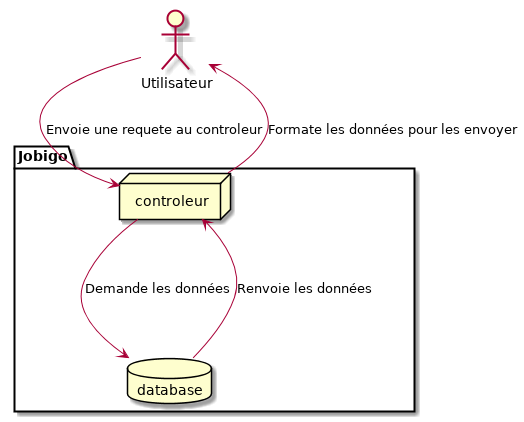
\includegraphics[scale=0.5]{jobigo}
            \caption{Plan de l'architecture}
            \label{fig:jobigo}
        \end{figure}

        \subsubsection{Les notifications push}
        Avec la démocratisation des smartphones, il y a eu une explosion de l'utilisation des notifications. C'est donc tout naturellement
        qu'il a fallu développer un mécanisme pour notifier les utilisateurs des événement relatif à jobigo.
        Les notifications push ne sont pas envoyée directement depuis le serveur, il faut faire appel à l'un des services proposé par Google (FCM, pour les appareils Android ou iOS) ou Apple (APNS, seulement pour iOS). Dans le cadre de jobigo, il a été décidé d'utiliser conjointement FCM et APNS.
        La figure \ref{fig:notification} résume le principe de fonctionnement des notifications push.

        \begin{figure}
            \centering
            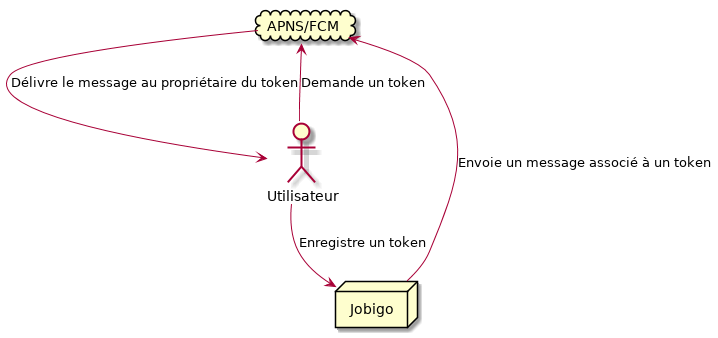
\includegraphics[scale=0.5]{notification}
            \caption{Fonctionnement des notifications push}
            \label{fig:notification}
        \end{figure}

        Un token est simplement un identifiant pour un appareil, un smartphone
        par exemple. Intuitivement on voudrait pourtant envoyer un message à
        une addresse qui identifie directement le smartphone d'un utilisateur,
        comme son addresse IP par exemple. Cependant procéder comme tel
        introduirait plusieurs problèmes~:
    \begin{itemize}
        \item L'IP n'est pas fixe (surtout avec un mobile) : il faudrait garder
            une trace des changement et forcer l'application à mettre à jour l'addresse IP à chaque
            changement : \textbf{c'est un traitement lourd}
        \item Si la sécurité du site est compromise, les addresses IP de tous
            les utilisateurs sont compromises : \textbf{c'est grave}
    \end{itemize}
        utiliser un token permet de déléguer toute la gestion des notification à un service externe, qui lui s'occupera des deux problèmes
        cités précédemment.


        \subsubsection{Problèmes rencontrés}
        L'un des principales difficultés que j'ai eu sur ce projet était l'utilisation de technologies qui étaient nouvelles pour moi.
        Les deux premières semaines ont donc été assez lourdes, puisqu'il a fallu que j'apprenne ce qu'était par exemple un token JWT pour l'authentification des utilisateurs, que je comprenne comment Docker était utilisé pour simplifier le déploiement du projet.

        Une autre difficulté qui est apparue vers la fin du projet a été le traitement asyncrone des notifications. En effet, envoyer des notifications nécessite de se connecter à un service externe, d'attendre la réponse, puis renvoyer une réponse à l'utilisateur. Seulement l'utilisateur n'a pas d'intérêt à attendre que google confirme que la notification a été envoyée. Normalement ce problème ce règle en exécutant ce traitement en arrière plan. Seulement php ne permet pas de le faire de manière simple.

        \subsection{Smart ULD}
        Une fois ce projet livré, j'ai été assigné à un autre projet.
        Le client en question développe un projet permettant de suivre des container
        à bord des avions, et notamment suivre leur geolocalisation.
        Pour que ce flux de données soit correctement acheminé, une architecture à base de micro-services
        avait déjà été prototypée par le client. Le but pour Siclo était donc à
        partir du prototype, de 
        redévelopper un ensemble de micro-service un peu plus robustes. Un
        résumé de l'architecture est disponible figure~\ref{fig:overview}.

        \begin{figure}
            \centering
            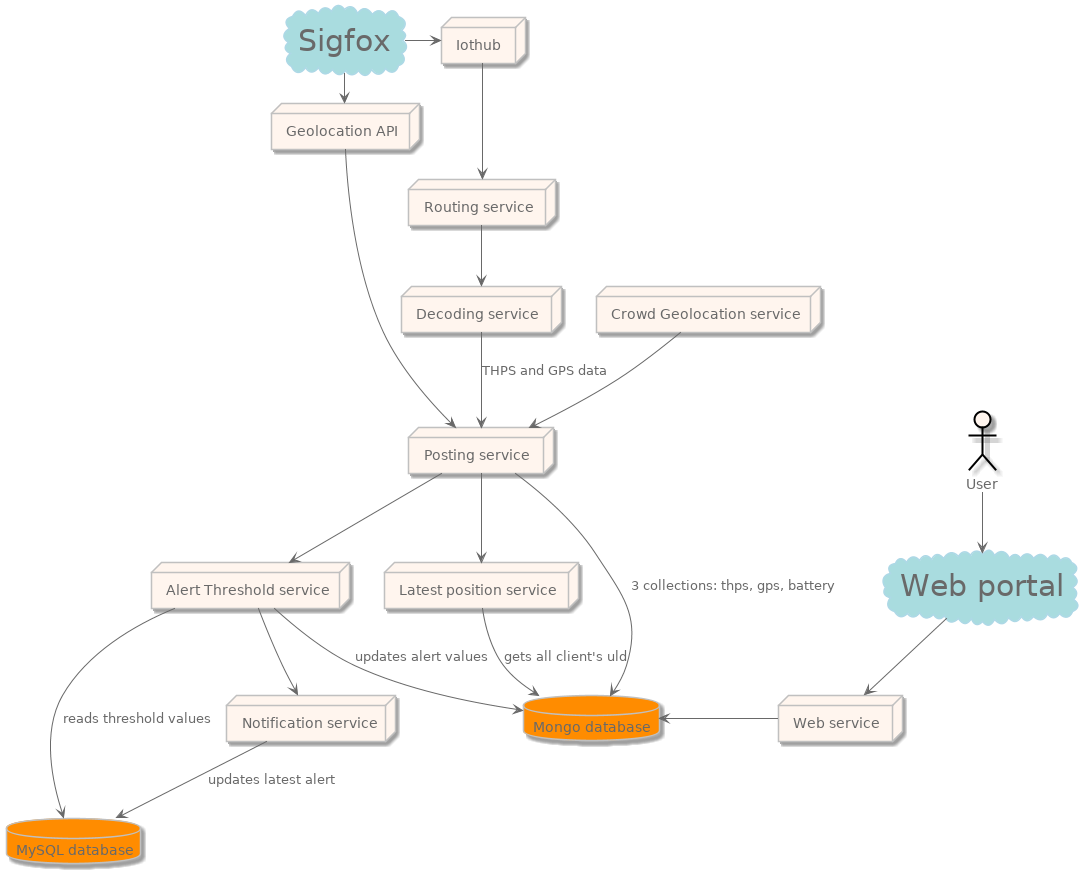
\includegraphics[scale=0.4]{servicesOverview}
            \caption{Plan de l'architecture}
            \label{fig:overview}
        \end{figure}

        \subsubsection{Decoding Service}
        C'est le premier service que j'ai dû implémenter. 
        Les données des divers capteurs arrivent par ce service. Deux types de
        capteurs sont utilisés, l'un envoit des données de géolocalisation,
        l'autre envoit des données physique\footnote{température, pression,
        humidité, choc (shock): THPS.}. Il a alors la charge décoder un message
        binaire, puis d'en déterminer le type\footnote{GPS ou THPS}. ce service
        sert principalement à mettre en forme les données en \gls{json}, puis
        les envoyer à un autre micro-service. dans le cas où les données ne
        sont pas conformes, les données sont refusés, et le message est ignoré.
        Le principe de ce service est résumé par l'algorithme la figure
        \ref{fig:algo_decoding}.
        En sortie du micro-service, il ne faut pas trouver de données
        incohérentes, qui viendrait alors 
        polluer la base de données.

        \begin{figure}
            \centering
            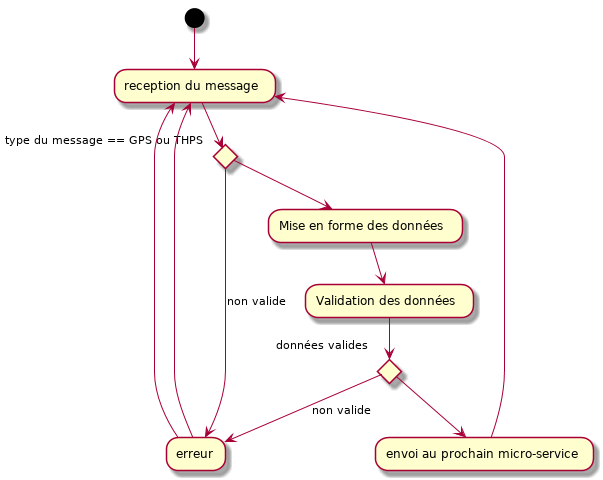
\includegraphics[scale=0.5]{algo_decoding}
            \caption{Plan de l'architecture}
            \label{fig:algo_decoding}
        \end{figure}

        \subsection{Mynabes}\label{subsec:mynabes}



\end{document}
